%\RequirePackage{flashmovie}
\documentclass{beamer}
\usepackage{graphicx}
%\usepackage{multimedia}
\usepackage{media9}

\definecolor{uoanavy}{RGB}{0,60,127}

\usetheme{Frankfurt}
\usecolortheme{orchid}
\setbeamertemplate{navigation symbols}{}
%\setbeamercolor{structure}{fg=uoanavy}

\usepackage{pgfplots}
\usepackage{pgfplotstable}
\pgfplotsset{compat=newest,
             jitter/.style={
                 x filter/.code={\pgfmathparse{\pgfmathresult+rnd*#1-#1/2}}
             },
             jitter/.default=0,
             select coords between index/.style 2 args={
                 x filter/.code={
                     \ifnum\coordindex<#1\def\pgfmathresult{}\fi
                     \ifnum\coordindex>#2\def\pgfmathresult{}\fi
                 }
             }
 }

\usepackage{doi}

\usepackage{animate}

% \usepackage{enumitem}
% \setlist[itemize]{label=$\triangleright$}

\title{Implementing Hamiltonian Monte Carlo for Efficient Bayesian Evolutionary Analysis}
\author{Arman Bilge \\ \small\texttt{abil933@aucklanduni.ac.nz}}

\institute{Computational Evolution Group \\ The University of Auckland}
\date{21 October 2015}

\usepackage{mathtools}
\newcommand{\dd}{\, \mathrm{d}}
\renewcommand{\vec}[1]{\ensuremath{\boldsymbol{\mathbf{#1}}}}
\newcommand{\mat}[1]{\ensuremath{\boldsymbol{\mathbf{#1}}}}
\newcommand{\op}[1]{\ensuremath{\boldsymbol{\mathbf{#1}}}}
\newcommand{\norm}[1]{\ensuremath{\mathcal{N}\left(#1\right)}}

\begin{document}

    \frame{\titlepage}

    \section{Introduction}

    \stepcounter{subsection}
    \begin{frame}{Motivation}

        \begin{itemize}

            \item Bayesian statistics has \textbf{transformed evolutionary biology}
            \begin{itemize}
                \item Divergence dating and clock rate estimation
                \item Inference of demographics and population history parameters
                \item Phylodynamic and epidemiological parameters
            \end{itemize}

            \item Want to \textbf{sample phylogenetic tree and model parameters} according to their probability given the data $P\left(\mathcal{T}, \theta \mid D\right)$

            \item Need a way to \textbf{efficiently explore} different models

        \end{itemize}

    \end{frame}

    \stepcounter{subsection}
    \begin{frame}{Current State-of-the-Art}
        \begin{itemize}
            \item Metropolis--Hastings Markov chain Monte Carlo (\textbf{MCMC})
            \item Imagine a robot taking a \textbf{random walk}
            \item Poor efficiency \pause
            \item \textbf{But suppose we gave our robot a pair of skis...}
        \end{itemize}
    \end{frame}

    \stepcounter{subsection}
    \begin{frame}{Cooker, an Aspiring Skier}
        \centering
        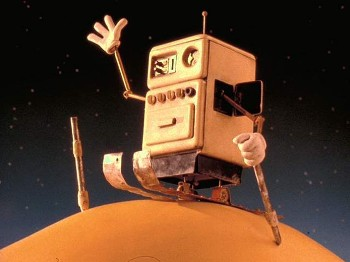
\includegraphics[width=0.75\textwidth]{skier}
    \end{frame}

    \section{Methods}

    \stepcounter{subsection}
    \begin{frame}{Physics Primer (Hamiltonian Dynamics)}
        \begin{columns}
            \begin{column}{.5\textwidth}
                \begin{definition}
                    Let
                    \small
                    \begin{itemize}
                        \item $\vec{q}$ be the robot's position
                        \item $\vec{v}$ be its velocity
                        \item $\mat{M}$ be its mass
                        \item $U\left(\vec{q}\right)$ be its potential energy
                        \item $K\left(\vec{p}\right)$ be its kinetic energy
                    \end{itemize}

                    \normalsize
                    Then the Hamiltonian $\mathcal{H}$ is
                    \begin{equation*}
                        \mathcal{H}\left(\vec{q},\vec{p}\right) = U\left(\vec{q}\right) + K\left(\vec{p}\right)
                    \end{equation*}
                \end{definition}
                \visible<2>{
                    \begin{itemize}
                        \item $\mathcal{H}$ is conserved
                        \item Simulates robot's motion
                    \end{itemize}
								}
            \end{column}
            \begin{column}{.5\textwidth}
            \centering
            	\begin{tikzpicture}
							 \node at (0, 0) {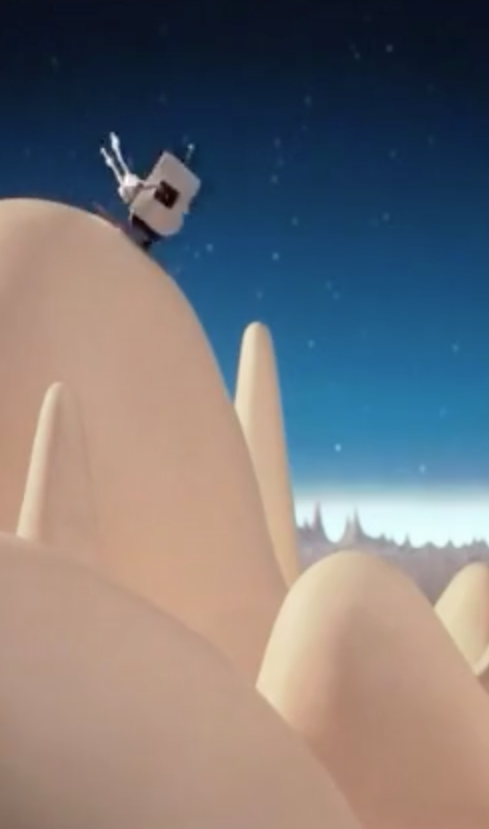
\includegraphics[width=0.75\textwidth]{primer}};
							 \draw[thick,<-] (-1,1.2) -- (-1, -3);
							 \node at (-0.5, -1) {$U\left(\vec{q}\right)$};
								\draw[thick,->] (-2,-3.2) -- (2, -3.2);

							 \node at (0, -2.9) {$\vec{q}$};
								\draw[thick,->,white] (-0.5,1.5) -- (0, 1);
								\node[white] at (0.8, 1.35) {$\vec{p}=\mat{M}\vec{v}$};
								
								\node[white] at (0, 3) {$K\left(\vec{p}\right) = \frac{1}{2}\vec{p}^T \mat{M}^{-1} \vec{p}$};
							 \end{tikzpicture}
            \end{column}
        \end{columns}
    \end{frame}

    \stepcounter{subsection}
    \begin{frame}{Hamiltonian Moves}
    \textbf{Flip direction}
    
    \centering
    \includemedia[
  width=0.75\textwidth,height=0.5625\linewidth,
  activate=pageopen,
  transparent,
  addresource=flip.mp4,
  flashvars={
   source=flip.mp4     % same path as in addresource!
   &loop=true           % loop video
   &autoplay=true
   &scaleMode=letterbox % preserve aspect ratio
  }
]{}{VPlayer9.swf}

    %    \movie[autostart,loop,width=0.75\textwidth,height=0.5625\textwidth]{flip}{flip.avi}
    \end{frame}
    
    \stepcounter{subsection}
    \begin{frame}{Hamiltonian Moves}
    \textbf{Ski!}
    
        \centering
    \includemedia[
  width=0.75\textwidth,height=0.5625\linewidth,
  activate=pageopen,
  transparent,
  addresource=ski.mp4,
  flashvars={
   source=ski.mp4     % same path as in addresource!
   &loop=true           % loop video
   &autoplay=true
   &scaleMode=letterbox % preserve aspect ratio
  }
]{}{VPlayer9.swf}

    \end{frame}

    \stepcounter{subsection}
    \begin{frame}{Hamiltonian Moves}
    \textbf{Push in a random direction}
    
                \centering
                    \includemedia[
  width=0.75\textwidth,height=0.5625\linewidth,
  activate=pageopen,
  transparent,
  addresource=random.mp4,
  flashvars={
   source=random.mp4     % same path as in addresource!
   &loop=true           % loop video
   &autoplay=true
   &scaleMode=letterbox % preserve aspect ratio
  }
]{}{VPlayer9.swf}

    \end{frame}

    \stepcounter{subsection}
    \begin{frame}{Hamiltonian Monte Carlo}
    
    \textbf{How do we make a stats problem into a physics problem?}
    \pause
    \begin{itemize}
    	\item Every location $\vec q$ maps to some model parameters
			\item Elevation at $\vec q$ is $-\log{P\left(\mathcal{T}, \theta \mid D\right)}$
    	\item Locations with \textbf{high elevation} have \textbf{low probability}
			\item Locations with \textbf{low elevation} have \textbf{high probability}
			\item Done!
    \end{itemize}
    
    \end{frame}

    \stepcounter{subsection}
    \begin{frame}{Hamiltonian Monte Carlo}

        \textbf{Running a physics simulator seems like a lot of work! \\ Why should we bother?}

        \pause

        \begin{theorem}[Creutz 1988]
            Consider a model with $n$ variables. \\
            Then (under simplifying assumptions) the computation time is
            \begin{itemize}
                \item $\mathcal{O}\left(n^2\right)$ for MCMC; and
                \item $\mathcal{O}\left(n^\frac{5}{4}\right)$ for HMC.
            \end{itemize}
        \end{theorem}

        \pause

        In practice this means \textbf{doubling the model complexity} increases computation time by
        \begin{itemize}
            \item \textbf{4x} for MCMC
            \item \textbf{$<$2.5x} for HMC!
        \end{itemize}

    \end{frame}

    \section{Results}

    \stepcounter{subsection}
    \begin{frame}{The Phylogenetic Ski Slope}

                \centering
                \animategraphics[autoplay,palindrome,controls]{15}{trajectory_}{000}{299}
      \end{frame}

    \stepcounter{subsection}
    \begin{frame}{Performance of HMC vs. MCMC}

        For $\left\{8,16,32,64\right\}$ taxa:

        \begin{enumerate}
            \item Simulated 100 datasets under Yule and HKY models
            \item Estimated node heights with optimally-tuned HMC/MCMC
            \item Measured efficiency as ESS of tree length per unit time
            (Effective Sample Size is \# of independent samples)
            \item Compared efficiency of HMC versus MCMC
        \end{enumerate}

    \end{frame}

    \stepcounter{subsection}
    \begin{frame}{Performance of HMC vs. MCMC}
        \centering
        \begin{tikzpicture}
            \begin{semilogxaxis}[width=0.9\textwidth,
                                 xtick={8,16,32,64},
                                 ytick={1,4,8,...,20},
                                 extra y ticks=1,
                                 extra y tick labels=,
                                 extra y tick style={ grid=major, major grid style={thick} },
                                 log ticks with fixed point,
                                 xlabel=Number of Taxa,
                                 ylabel=Relative Efficiency of HMC,
                                 clip mode=individual
                         ]
                \addplot+[uoanavy, only marks, mark size=1, mark options={fill=uoanavy}, jitter=0.25] table {performance.dat};
                \draw[red, thick] (7, 4.21355) -- (9.14285714285714, 4.21355);
                \draw[red, thick] (14, 4.776769) -- (18.28571, 4.776769);
                \draw[red, thick] (28, 5.342736) -- (36.57143, 5.342736);
                \draw[red, thick] (56, 5.547638) -- (73.14286, 5.547638);
            \end{semilogxaxis}
        \end{tikzpicture}
    \end{frame}

    \section{Conclusion}

    \stepcounter{subsection}
    \begin{frame}{Concluding Remarks}
        \begin{block}{Conclusions}
            \begin{itemize}
                \item HMC \textbf{consistently out-performed} MCMC
                \item On average, HMC was \textbf{5x more efficient} than MCMC
                \item Open source implementation at \texttt{http://github.com/armanbilge/B3/tree/hamilton}
            \end{itemize}
        \end{block}
        \break
        \begin{block}{Future Work}
            \begin{itemize}
                \item Inferring parameters for other evolutionary models
                \item Moving between tree topologies
                \item Automatic tuning of HMC for optimal performance
                \item Implementing and testing more sophisticated flavors of HMC
            \end{itemize}
        \end{block}
    \end{frame}

    \stepcounter{subsection}
    \begin{frame}{Acknowledgements}
        \begin{block}{Thanks to}
            \begin{itemize}
                \item Tim Vaughan and Alexei Drummond
                \item Members of the Computational Evolution Group
                \item Allan Wilson Centre Summer Scholarship
                \item New Zealand eScience Infrastructure
            \end{itemize}
        \end{block}
        \begin{block}{References}
            \footnotesize
            M Creutz. \textit{Physical Review D} 38.4 (1988). \texttt{\doi{10.1103/PhysRevD.38.1228}} \\
            RM Neal. \textit{Handbook of Markov Chain Monte Carlo} (2011).
        \end{block}
    \end{frame}

\end{document}
